\begin{center}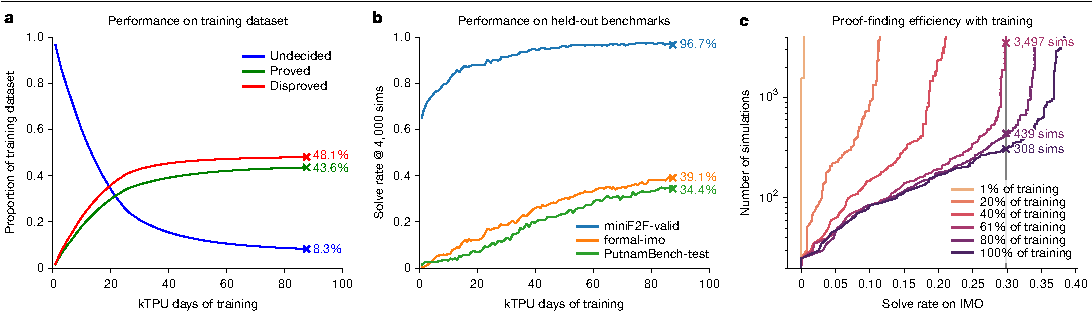
\includegraphics[width=\linewidth]{../papers/translations/alphaproof/assets/fig3.pdf}\end{center}
\phantomsection
\noindent\textbf{原文图 3. AlphaProof 在主 RL 中的学习进程.}\paperlabel{3}{alphaproof-fig3}
a, 训练集 (自动形式化问题) 上的表现演变. 曲线显示随 Google Cloud TPU v6e 计算增加, 起始实例中已证明 (绿)、已反驳 (红)、未判定 (蓝) 的比例. b, 训练期间留出集 miniF2F-valid、formal-imo、PutnamBench-test 在 4,000 次模拟 (sims) 的解题率. c, 主 RL 不同阶段达到历史 IMO 某个解题率所需的树搜索模拟数, 使用对数尺度. 每条曲线对应不同训练阶段检查点. 后期智能体不仅更强, 也更高效, 达到同一解题率所需搜索显著减少. 例如, 最终模型仅 300 次模拟就解约 $30\%$ 的问题, 早期模型即使更多搜索也无法达到该水平.

\noindent\textbf{图中文字对应.} Performance on training dataset: 训练集表现; Proportion of training dataset: 训练集比例; Undecided、Proved、Disproved: 未判定、已证明、已反驳; kTPU days of training: 训练计算 (千 TPU 日); Performance on held-out benchmarks: 留出集表现; Solve rate @ 4,000 sims: 4,000 次模拟解题率; Proof-finding efficiency with training: 随训练改变的寻证效率; Number of simulations: 模拟次数; Solve rate on IMO: IMO 解题率. 1\%、20\%、40\%、61\%、80\%、100\% of training 分别为对应训练进度. 各标注百分数与模拟数均保持原值.
